\documentclass[12pt]{article}
\usepackage{graphicx}
\usepackage{tabularx}
\usepackage[section]{placeins}
\usepackage[section]{placeins}
\usepackage[section]{placeins}
\usepackage[section]{placeins}
\usepackage[section]{placeins}
\usepackage{float}
\usepackage{siunitx}
%
% Title[Enter title of the experiment here]
\title{EE230: Lab 7\\
Active filters}

% Packages
\usepackage[RPvoltages]{circuitikz}
 
 
\begin{document}
 

% Author[Enter details of author here]
\author{Mudavath vishnuvardhan, 200070044}

% begin the document.
\begin{document}

% make a title page.[this creates title page]
\maketitle



\section{Overview of the experiment} %[This segment creates Section as seen in document]

\subsection{Aim of the experiment}%[This segment creates sebsections under the same section]
To perform in-lab experiments for plotting the Sallen-Key Active low pass, high pass and band pass filter and find the cutoff frequency.


\subsection{Methods}
\subsubsection{Active Low Pass & High pass filter}
Sallen-Key is a second-order(two pole). Its also known as Voltage-controlles voltage source filter which happens to be a low-pass filter and high-pass filter based on the configuration of R and C where filter is of Butterworth. One RC circuit consits of \(R_{A}\) and \(C_{A}\), and the second circuit consits of \(R_{B}\) and $C_{B}$.\\
One feature of this type of filter is that the capacitor $C_{A}$ provides feedback for shaping the response near the edge of the passband
\begin{figure}[H]
\centering
\caption{Lowpass Filter}
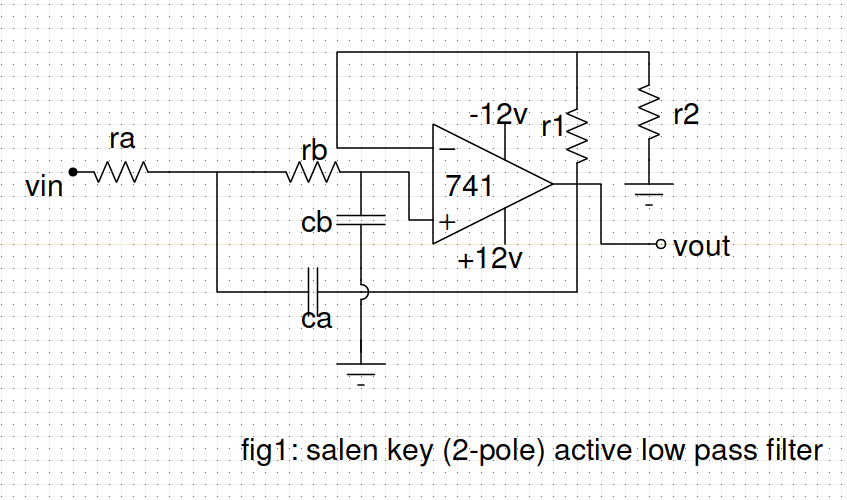
\includegraphics[scale = 0.4]{low-pass.png}
\end{figure}
\begin{figure}[H]
\centering
\caption{Highpass Filter}
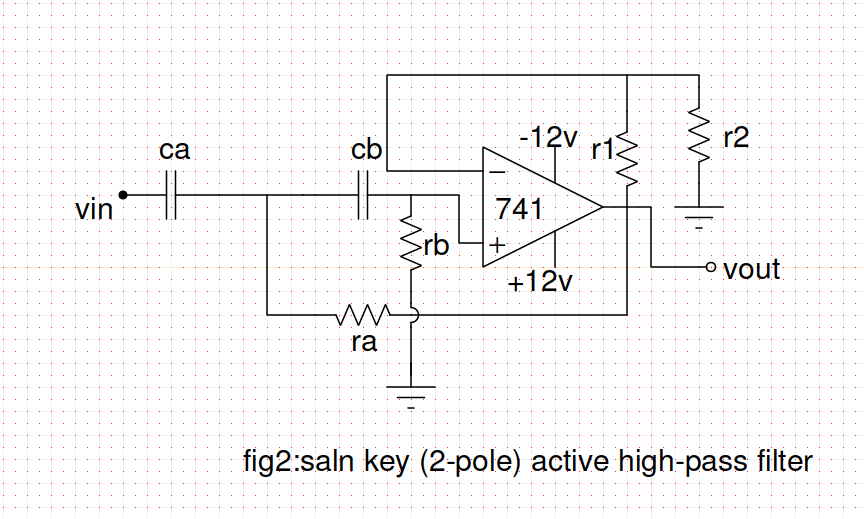
\includegraphics[scale = 0.4]{high-pass.png}
\end{figure}

Critical frequency is given by $f_{c}=\frac{1}{2\pi\sqrt{R_{A}R_{B}C_{A}C_{B}}}$\\
But as $R_{A}=R_{B}$ and $C_{A}=C_{B}$, hence, $f_{c}=\frac{1}{2\pi{RC}}$
\subsection{Multiple-feedback Active Band-Pass Filter}
Multiple-feedback band-pass filter has two feedback paths through $R_{2}$ and $C_{1}$. Components $R_{1}$ and $C_{1}$ provide the low-pass response, and $R_{2}$ and $C_{2}$ provide the high-pass response, the maximum gain $A_{o}$ which occurs at the center frequency whose expression is recorgnised as $R_{1}$ and $R_{3}$ in parallel combination with $C_{1}$ feedback path, so $f_{o}=\frac{1}{2\pi\sqrt{(R_{1}||R_{3)R_{2}C_{1}C_{2}}$,\\ but $C_{1}=C_{2}=C$, hence $f_{o}=\frac{1}{2\pi C}\sqrt{\frac{R_{1}+R_{3}}{R_{1}R_{2}R_{3}}}}}$.

\begin{figure}[H]
\centering
\caption{Equivalent Circuit}
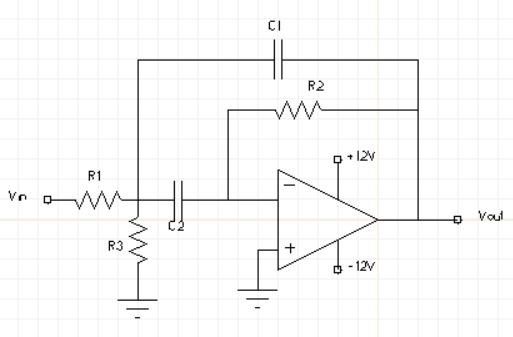
\includegraphics[scale = 0.4]{fig3.jpeg}
\end{figure}





\section{Experimental Results}
\subsection{Active Low pass}
\begin{figure}[H]
\centering
\caption{Lowpass Filter Data}
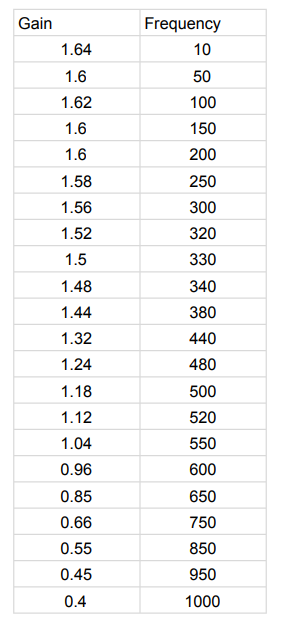
\includegraphics[scale = 0.5]{Readings1.png}
\end{figure}
\begin{figure}[H]
\centering
\caption{Lowpass Filter Plot}
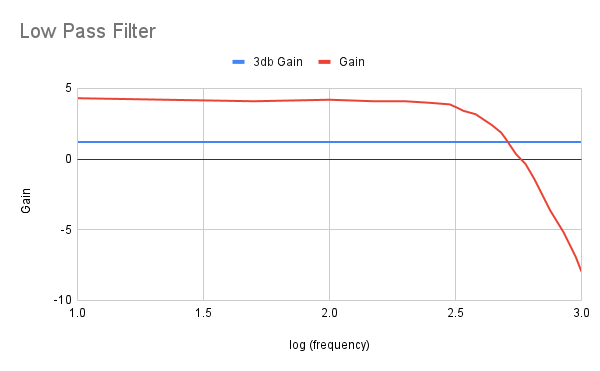
\includegraphics[scale = 0.5]{Low Pass Filter.png}
\end{figure}
\subsection{Active High pass}
\begin{figure}[H]
\centering
\caption{Highpass Filter Data}
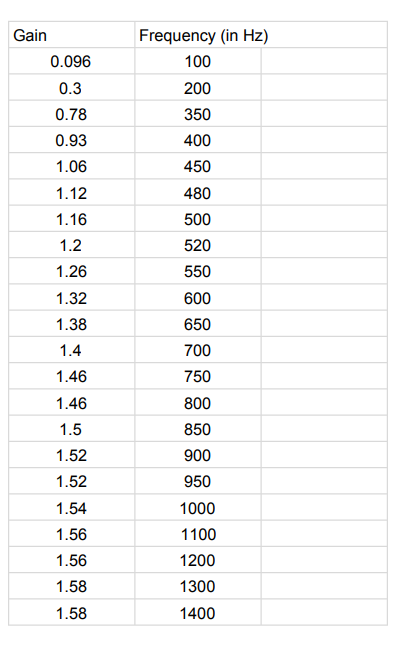
\includegraphics[scale = 0.5]{Readings2.png}
\end{figure}
\begin{figure}[H]
\centering
\caption{Highpass Filter Plot}
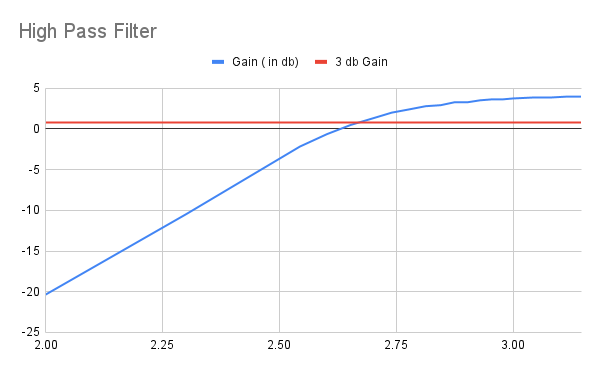
\includegraphics[scale = 0.5]{High Pass Filter.png}
\end{figure}
\subsection{Band-pass}
\begin{figure}[H]
\centering
\caption{Bandpass Filter Data}
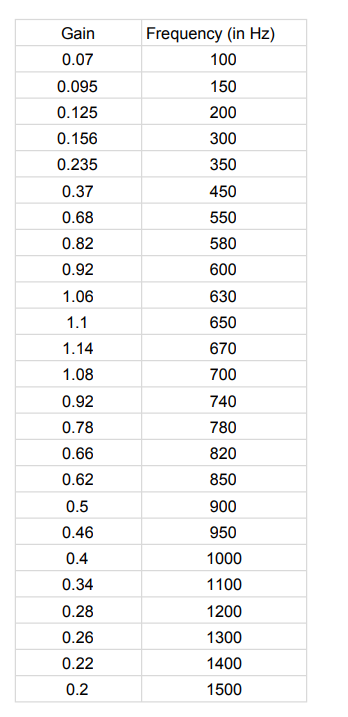
\includegraphics[scale = 0.4]{Readings3.png}
\end{figure}
\begin{figure}[H]
\centering
\caption{Bandpass Filter Plot}
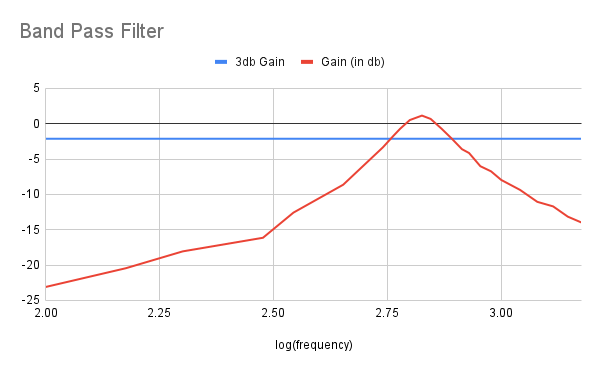
\includegraphics[scale = 0.4]{Band Pass Filter.png}
\end{figure}

\section{Experiment Completion Status}
All required parts completed\\
Parts :\\
1. Active Low-pass filter\\
2. Active High-pass filter\\
3. Active Band-pass filter\\
\end{document}
\end{document}
